\section*{Question 1}

{\bfseries Take at your own choice several keypoints that have been
detected at different scales. Using the theory given in the lectures, comment on
the reasons of why do you think that a keypoint has been detected at that position
and at that particular scale. You may repeat the experiment with another image
(such as 'river1') to understand what a significant keypoint is.}

When running the keypoint detection function \texttt{vl\_sift} on the image \texttt{river1}, 1816 keypoints are detected. We hand-picked several keypoints to demonstrate why they were picked. The selected keypoints can be seen in figure \ref{fig:keypoint01}. Keypoints were selected in different areas of the image and at different scales, ranging from 2.3 for keypoint D to 13.6 for keypoint A. While this is just a small part of all detected keypoints, they represent a variety of different points at different locations with different scales.

\begin{figure}[!hbt]
  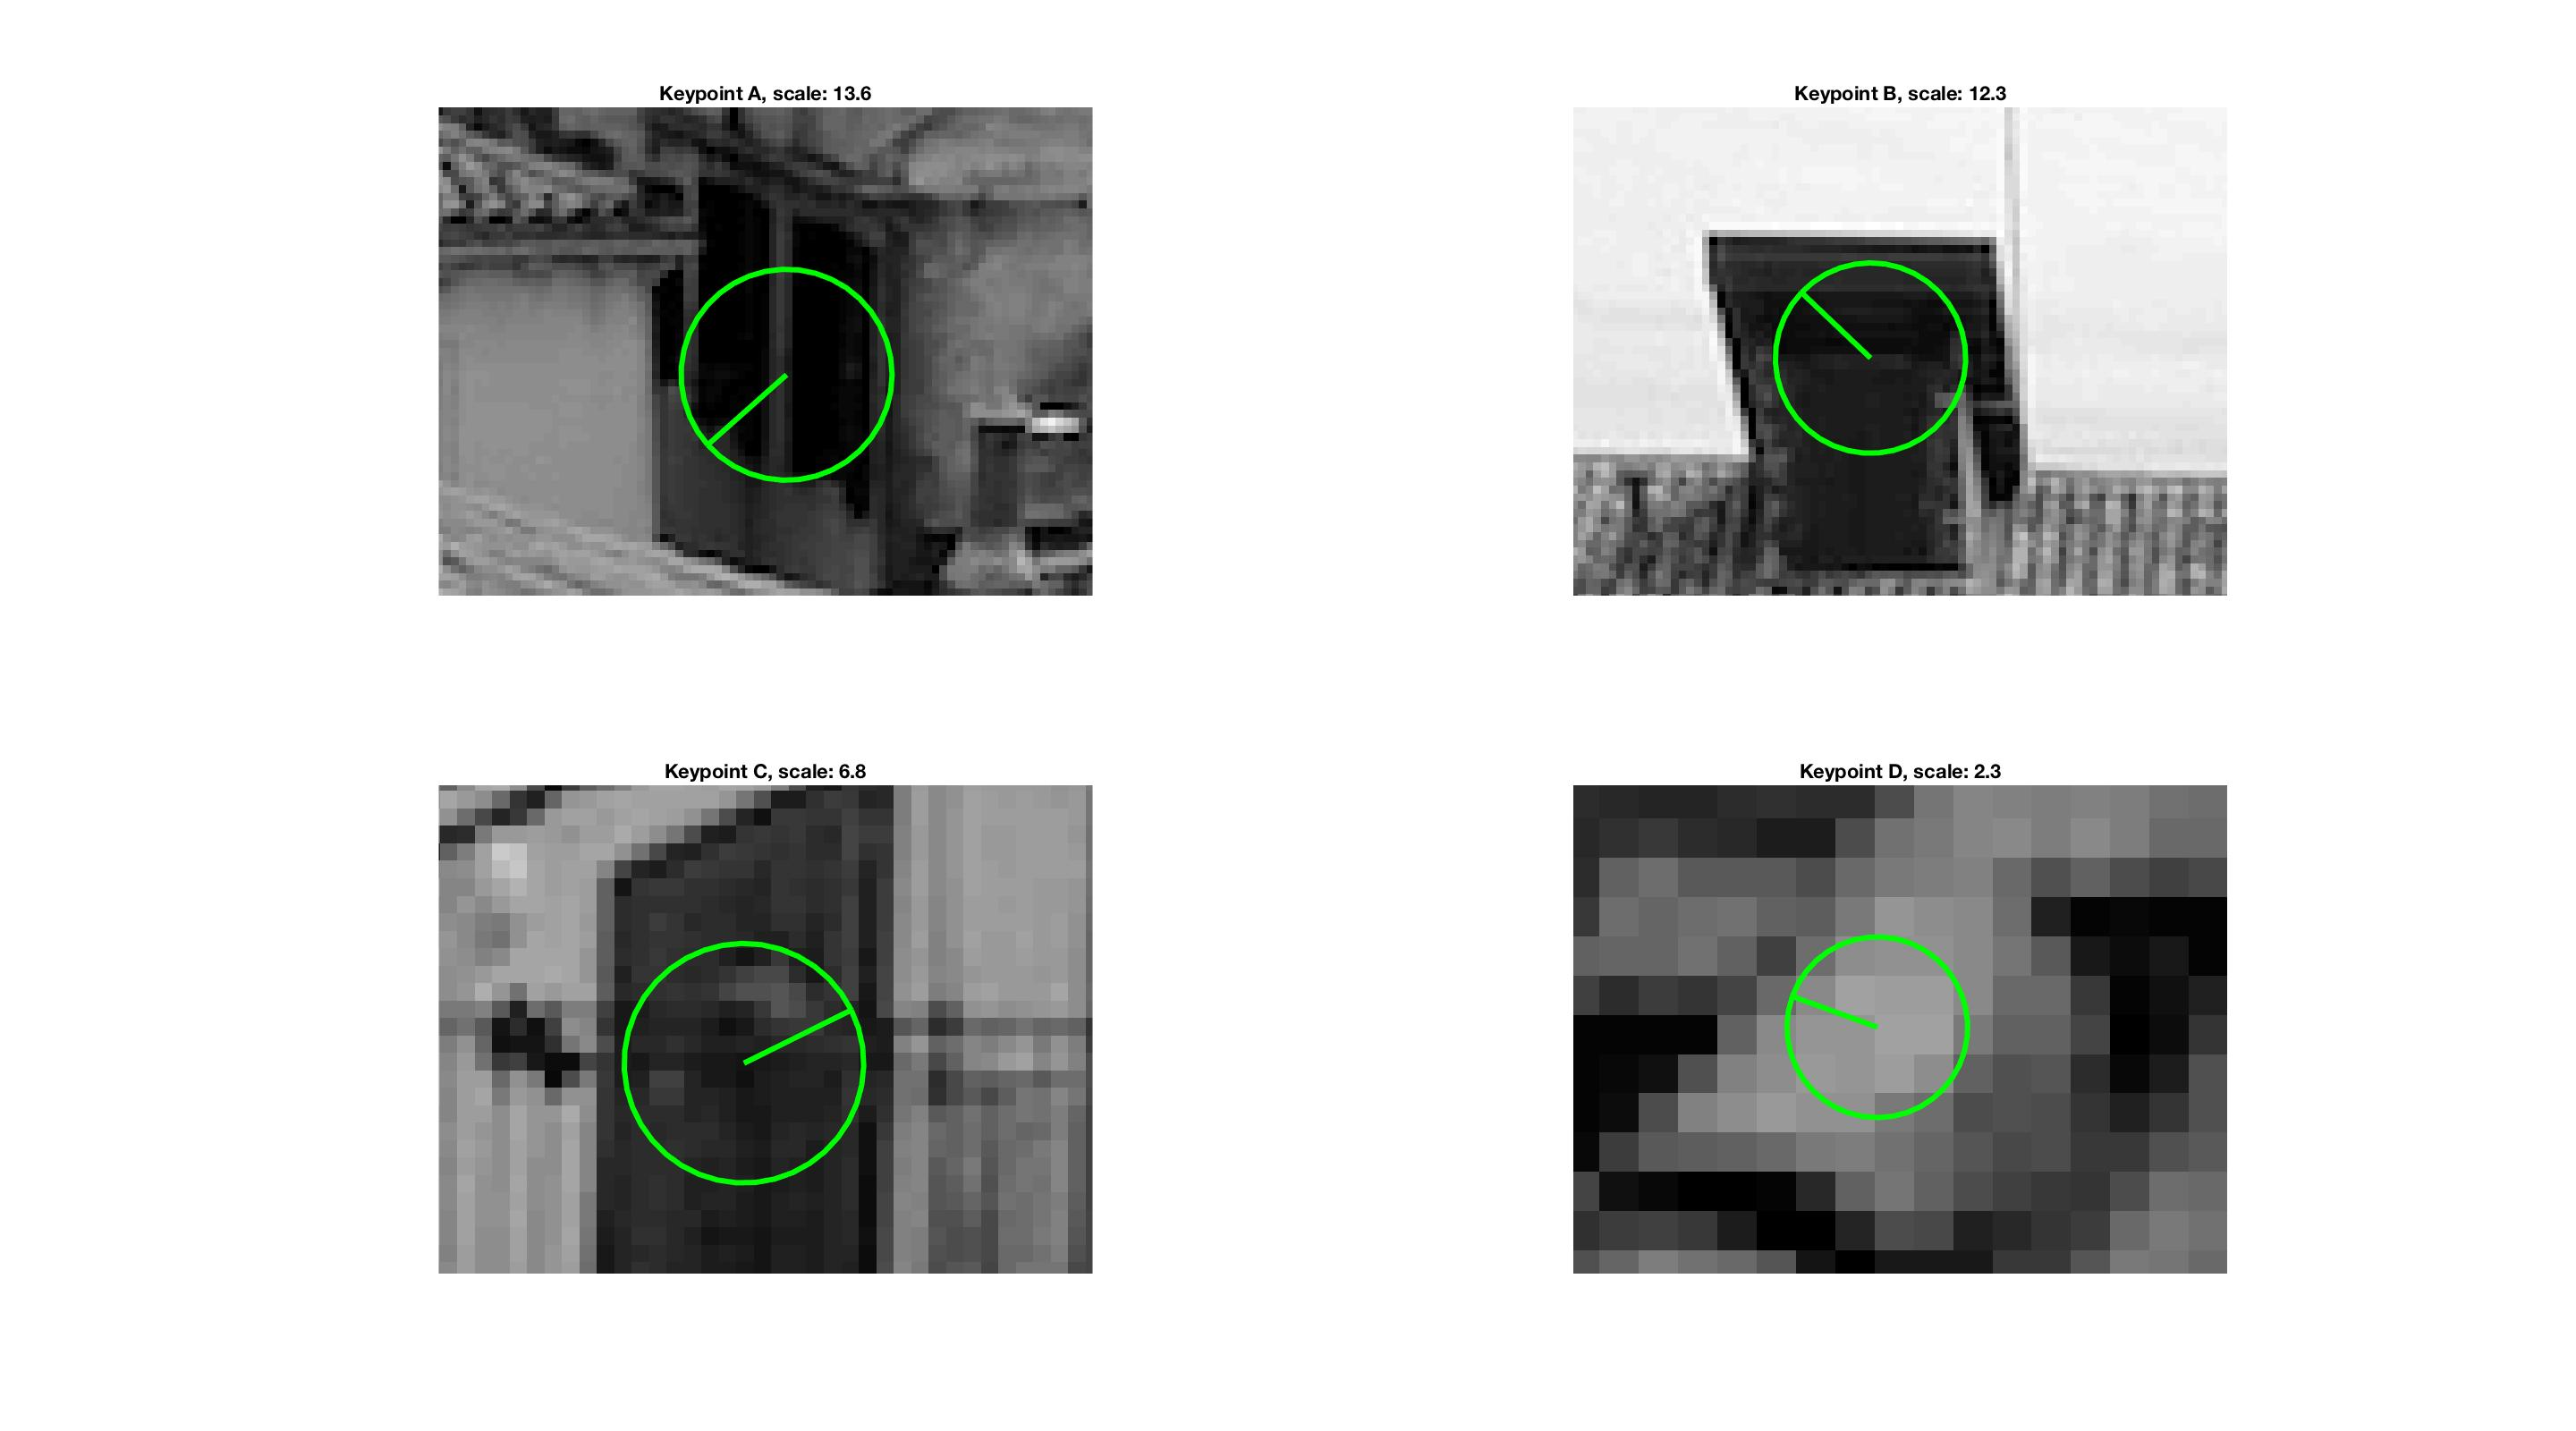
\includegraphics[width=\textwidth]{img/keypoint01}
  \caption{Example keypoints}
  \label{fig:keypoint01}
\end{figure}

Keypoint A was detected at the position of a window on the corner of a house. The scale of 13.6 represents the width of this window. For this scale, there is a strong gradient around the selected keypoint, since the pixels around the window have a higher brightness.  

Keypoint B was selected at the position of a roof hatch. The gradient for this scale is strong since the ceiling around the hatch is much brighter. The scale of 12.3 more or less fits the width of the hatch, making it a strong candidate for a promising keypoint.

Similarly, keypoint C was detected at the position of a balcony door with a strong gradient between the dark door and the bright wall around it. Again, the scale of 6.8 corresponds to the door's width. 

Keypoint D is at a much smaller level with a scale of only 2.3. It is located on a tile of one of the roofs. As we can see after zooming in on its location, there is a strong edge between the bright part of the tile and the shade around it. The scale is similar to the width of the bright part and when calculating the difference of Gaussians at this scale there will be a extreme difference towards surrounding pixels in the scale space.